\documentclass{article}
\usepackage[english]{babel}
\usepackage{longtable}
\usepackage[top=1in, bottom=0.25in, left=1.25in, right=1.25in,includefoot,heightrounded]{geometry}
\usepackage{indentfirst}
\usepackage[utf8]{inputenc}
\usepackage{amsmath,amssymb}
\usepackage{graphicx,tikz}
\usepackage{hyperref}
\usepackage[colorinlistoftodos]{todonotes}
\usepackage[document]{ragged2e}
\usepackage{fancyhdr}
\usepackage{enumerate}
\usepackage{listings}
\usepackage{color}
\usepackage{flowchart}
\usepackage{hyperref}
\usepackage{graphicx}
\usetikzlibrary{arrows}

\usetikzlibrary{shapes.geometric, arrows}
\tikzstyle{startstop} = [rectangle, rounded corners, minimum width=3cm, minimum height=1cm,text centered, draw=black, fill=red!30]
\tikzstyle{decision} = [diamond, minimum width=4cm, minimum height=0.5cm, text centered, draw=black, fill=green!30]
\tikzstyle{process} = [rectangle, minimum width=3cm, minimum height=1cm, text centered, draw=black, fill=orange!30]
\tikzstyle{arrow} = [thick,->,>=stealth]
\tikzstyle{io} = [trapezium, trapezium left angle=70, trapezium right angle=110, minimum width=2cm, text width=4cm, minimum height=1cm, text centered, draw=black, fill=blue!30]

\pagestyle{fancy}
\fancyhf{}
\lhead{Myles Deslippe}
\rhead{Comp 3670 | Computer Networks}
\cfoot{\thepage}

\definecolor{MyDarkGreen}{rgb}{0.0,0.4,0.0}
\lstset{inputencoding=ansinew}
\lstset{breaklines=true} 

\begin{document}

\section*{\centering{Network Layer Overview}}

    \subsection*{Services and Protocols}
    \begin{itemize}
        \item To transport \textbf{segments} from the \textbf{sending host}, to the \textbf{receiving host} the following happens:
        \begin{enumerate}
            \item The \textbf{sender} \textbf{encapsulates segments} into \textbf{datagrams} and passes them to the \textbf{link layer}.
            \item The \textbf{receiver delivers segments} to the \textbf{transport layer protocol}. 
            \item A \textbf{router} is a piece of \textbf{network hardware} than manages \textbf{traffic between networks}.
            \begin{itemize}
                \item Routers work by examining the headers in \textbf{IP datagrams (Packets)}, and move the datagrams from \textbf{input ports} to \textbf{output ports}; with the goal of transfering datagrams along the end-end path.
                \item Routers work a the \textbf{Network Layer (Layer 3)}, and also use layers 1 and 2 to facilitate the data transfer.
                \item Routers us \textbf{Internet Protocol Addresses (IP Address)} to identify networks / hosts.
            \end{itemize}
        \end{enumerate}
    \end{itemize}

    \subsection*{Key Network-Layer Functions}
    \begin{itemize}
        \item One key network-layer function is \textbf{forwarding}, \textbf{forwarding} involves \textbf{moving packets} from a \textbf{rounter's input link} to the appropriate \textbf{output link}.
        \item Another key network-layer function is \textbf{routing}, \textbf{routing} involves \textbf{determining the route taken by packets} from the \textbf{source} to the \textbf{destination}.
        \begin{itemize}
            \item There are many routing algorithms that can be used the achieve this.
        \end{itemize}
    \end{itemize}

    \subsection*{The Data Plane vs The Control Plane}
    \begin{itemize}
        \item The \textbf{data plane} is a \textbf{local, per-router function} that \textbf{determines how packets} arriving on a router's input port \textbf{is forwarded to router's output port}.
        \item The \textbf{control plane} is a \textbf{network-wide} function, that \textbf{determines how packets} are \textbf{routed amongst routers} along end-end paths from \textbf{source host} to \textbf{destination host}.
        \begin{itemize}
            \item There are two control-plane approaches:
            \begin{enumerate}
                \item \textbf{Traditional routing algorithms} that are implemented in routers.
                \item \textbf{Software-defined networking (SDN)} that is implemented in remote servers.
            \end{enumerate}
        \end{itemize}
    \end{itemize}

    \subsection*{Per-Router Control PLane Software-Defined Networking (SDN) Control Plane}
    \begin{itemize}
        \item \textbf{Per-Router control plane} consits of a \textbf{routing algorithm} in \textbf{every router} that interacts with the \textbf{control plane}. Each router determines where to route the \textbf{packets}.
        \item \textbf{SDN} is composed of \textbf{remote controller computers}, that \textbf{install forwarding tables} in router. The routers then use these tables to forwards \textbf{packets}.
        \item[] \begin{center}
                    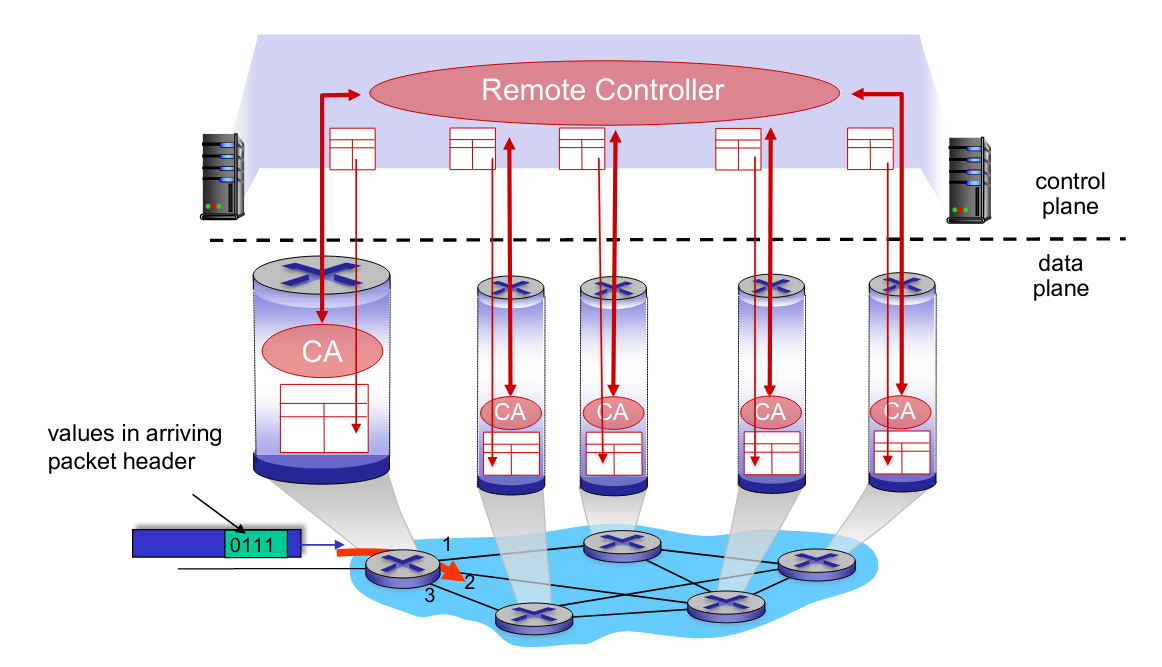
\includegraphics[width=\textwidth - 25pt]{images/Software-Defined-Networking.png}
                \end{center}
    \end{itemize}

    \subsection*{Network Service Models}
    \begin{itemize}
        \item Internet service models:
        \item[] 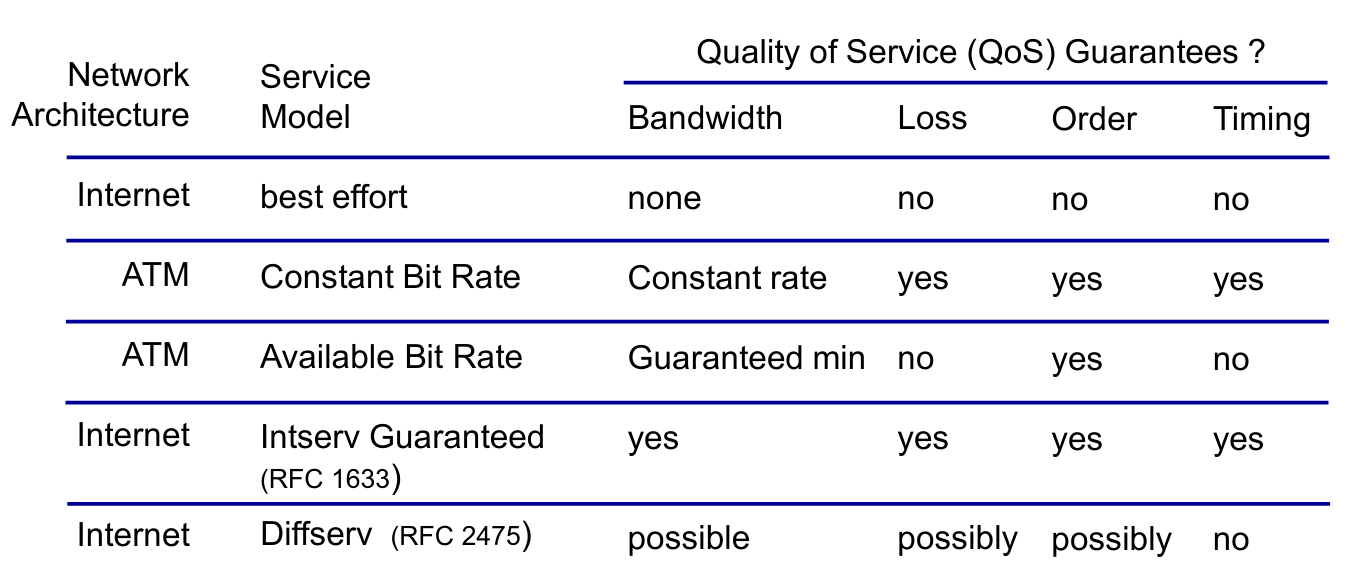
\includegraphics[width=\textwidth - 25pt]{images/Network-Service-Models.png}
        \item Though the \textbf{best effor service model} may not provide any guarantees, it allowed the internet to be widely deployed, and adopted. 
    \end{itemize}

\section*{\centering{Router Architecture Overview}}

    \subsection*{Routers}
    \begin{itemize}
        \item A \textbf{router} is a \textbf{networking device} that \textbf{forwards} and \textbf{router data packets} between \textbf{networks}.
        \item \textbf{Routers} have \textbf{input ports} and \textbf{output ports}, to \textbf{receive} and \textbf{forward} packets respectively.
        \item[] 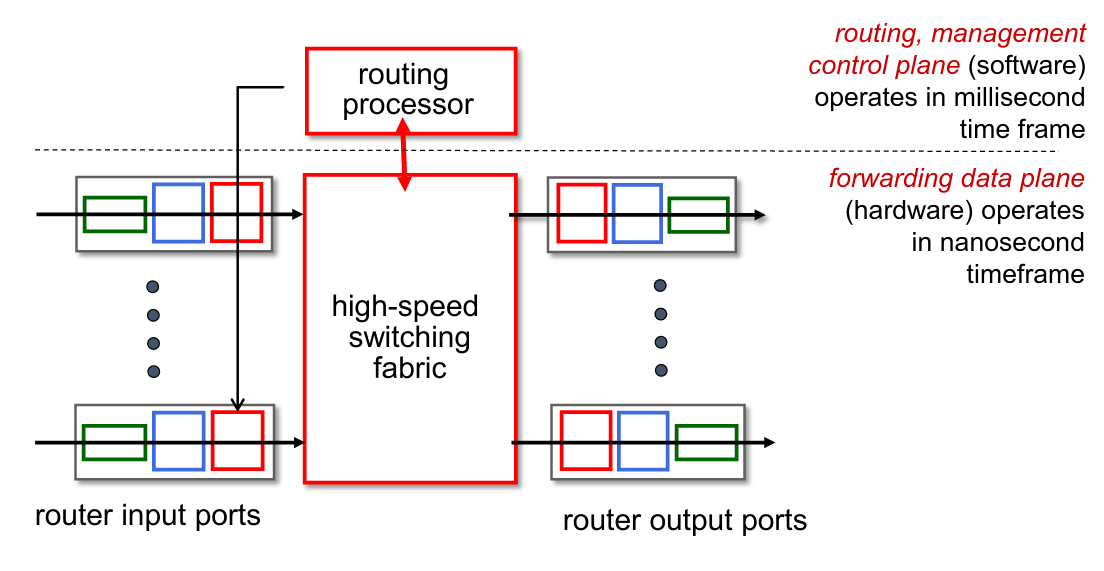
\includegraphics[width=\textwidth - 25pt]{images/Router-Overview.png}
        \begin{itemize}
            \item The green boxes represents the \textbf{physical layer}, the blue boxes represent the \textbf{link layer}, and the red boxes represent the \textbf{network layer}.
            \item The first red box continas a queue of packets that need to be forwarded, and the lookup table, that map headers to ports.
        \end{itemize}
        \item \textbf{Destination-based forwarding} is forwarding based only on the \textbf{destination IP Address} (traditional).
        \item \textbf{Generalized forwarding} is forwarding based on \textbf{any set of header field values}.
        \item The following is an example of a lookup table:
        \item[] 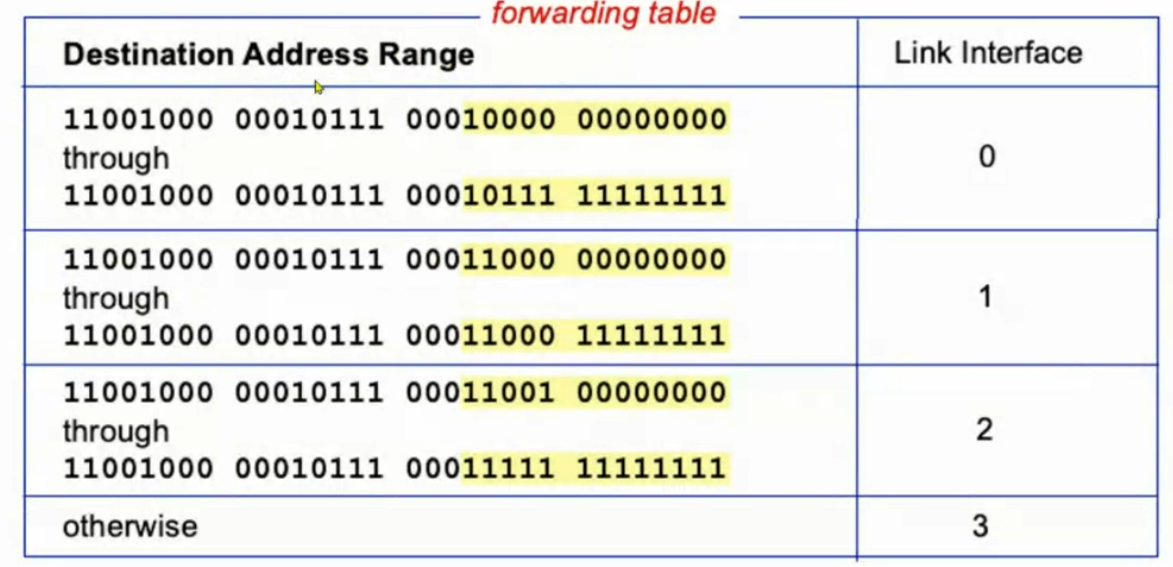
\includegraphics[width=\textwidth - 25pt]{images/Forward-Table.png}
        \begin{itemize}
            \item To determine which interface a an IP address should be mapped to, you see what address range has the longest prefix that matches the IP address of the packet that is being router.
        \end{itemize} 
    \end{itemize}

    \subsection*{Switching Fabrics}
    \begin{itemize}
        \item \textbf{Switching fabrics} are responsible for transfering the \textbf{packet} from the \textbf{input link} to the appropriate \textbf{output link}.
        \item The \textbf{switching rate} is the rate at which \textbf{packets can be trasnferred} from \textbf{inputs} to \textbf{outputs}.
        \item There are \textbf{three main types of switching fabrics}:
        \item[] 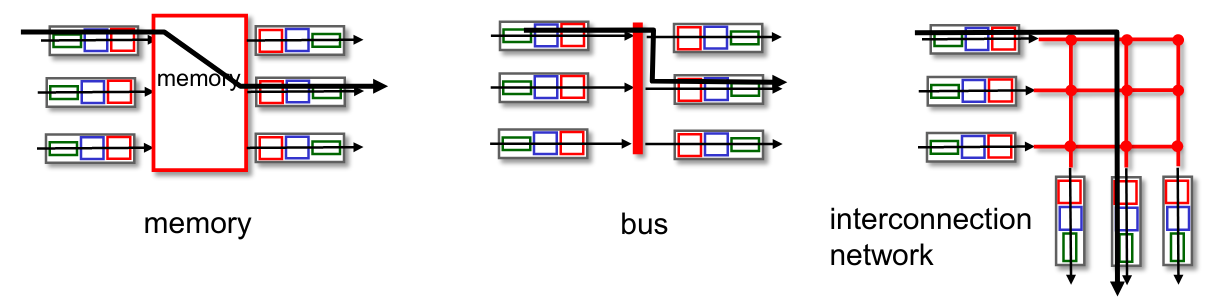
\includegraphics[width=\textwidth - 25pt]{images/Switching-Fabrics.png}
        \item With \textbf{memory switching}, the packets are copied to the \textbf{system's memory}. This limits the switching rate to the \textbf{memories bandwidth}. This type of switching is directly under the control of the \textbf{CPU}.
        \item With \textbf{bus switching}, the packets are delivered from the \textbf{input port's memory}, to the \textbf{output port's memory} directly. The switching speed is limited to the \textbf{speed of the bus} (which is much faster than memory switching). 
        \item With \textbf{interconnnection network switching}, is similar to the bus, except we can \textbf{transfer several packets in parallel}.
    \end{itemize}

    \subsection*{Input Port Functions}
    \begin{itemize}
        \item 
    \end{itemize}

\end{document}